\documentclass[11pt]{exam}

\oddsidemargin=0.25truein \evensidemargin=0.25truein
\topmargin=-0.5truein \textwidth=6.0truein \textheight=8.75truein

%\RequirePackage{graphicx}
\usepackage{comment}
\usepackage{verbatim}
\usepackage{booktabs}
\usepackage{graphicx}
\usepackage{hyperref}
\urlstyle{rm}   % change fonts for url's (from Chad Jones)
\hypersetup{
    colorlinks=true,        % kills boxes
    allcolors=blue,
    pdfsubject={ECON-UB233, Macroeconomic foundations for asset pricing},
    pdfauthor={Dave Backus @ NYU},
    pdfstartview={FitH},
    pdfpagemode={UseNone},
%    pdfnewwindow=true,      % links in new window
%    linkcolor=blue,         % color of internal links
%    citecolor=blue,         % color of links to bibliography
%    filecolor=blue,         % color of file links
%    urlcolor=blue           % color of external links
% see:  http://www.tug.org/applications/hyperref/manual.html
}

\renewcommand{\thefootnote}{\fnsymbol{footnote}}
\newcommand{\var}{\mbox{\it Var\/}}

\printanswers

% document starts here
\begin{document}
\parskip=\bigskipamount
\parindent=0.0in
\thispagestyle{empty}
{\large ECON-UB 233 \hfill Dave Backus @ NYU}

\bigskip\bigskip
%\centerline{\Large \bf Lab Report \#7:  Stochastic Processes}
\centerline{\Large \bf Lab Report \#7:  Dynamics in Theory and Data}
\centerline{Revised: \today}

\bigskip
{\it Due at the start of class.
You may speak to others, but whatever you hand in should be your own work.
Please include your Matlab code.}

\begin{questions}

%\begin{solution}
%Answers follow.  See Matlab code at the end for calculations.
%\end{solution}

%-----------------------------------------------------------------------
\question {\it Linear models.\/}
Consider the models
\begin{eqnarray*}
(a) &&  x_t \;\;=\;\; 0.9 x_{t-1} +  w_t \phantom{xxxxxxxxxxxxxxxxxxxxxxxxxxxxxxxxxxxx}\\
(b) &&  y_t \;\;=\;\; x(t) + 2 \\
(c) &&  x_t \;\;=\;\; 0 \cdot w_t + 1 \cdot w_{t-1} \\
(d) &&  x_t \;\;=\;\; \varphi x_{t-1} + w_t + \theta  w_{t-1} \\
(e) &&  x_t \;\;=\;\; 1.2 x_{t-1} + 0.1 x_{t-2} +  w_t
\end{eqnarray*}
[The idea behind (b) is to take $x_t$ from (a) and add 2.]

For each model,  answer the questions:
\begin{enumerate}
\item [(i)] Is it Markov?  For what definition of the state? %\\
\item [(ii)] What is the conditional distribution of of $x_{t+1}$ given
the state at date $t$? %\\
\item [(iii)] Is it stable?
\item [(iv)] If it's stable, what is the stationary distribution?
What is the autocorrelation function?
\end{enumerate}


\begin{solution}
All of these are Markov.
The state ($z_t$, say) is whatever you need to know at date $t-1$ to
know the conditional distribution of $x_t$.
\begin{parts}
\part This is an AR(1).
(i)~It's Markov with state $x_{t-1}$.
(ii)~Conditional distribution:  normal with mean $0.9 x_{t-1}$ and variance one.
(iii)~Yes, stable, because 0.9 is less than one in absolute value.
(iv)~The stationary distribution is normal with mean zero and variance
$1/(1-0.9^2) = 5.2632$.
The autocorrelation function is
\begin{eqnarray*}
    \rho(k) &=& 0.9^k .
\end{eqnarray*}
This includes $\rho(1) = 0.9$, $\rho(2) = 0.9^2 = 0.81$, and so on.

\part Still an AR(1).
(i)~Doing the substitution $x_t = y_t - 2$ gives us
\begin{eqnarray*}
    y_t &=& (1-0.9) \cdot 2 + 0.9 y_{t-1} + w_t .
\end{eqnarray*}
So it's Markov with state $y_{t-1}$.
(ii)~Conditional distribution:  normal with mean $0.2 + 0.9 y_{t-1}$ and variance one.
(iii)~Yes, stable, because 0.9 is less than one in absolute value.
(iv)~The stationary distribution is normal with mean two and variance
$1/(1-0.9^2) = 5.2632$.
All we've done here is shift the mean up by two.
The autocorrelation function doesn't depend on the mean, so it's the same
as before.

\part This is an MA(1).
(i)~It's Markov with state $w_{t-1}$.
(ii)~Conditional distribution:  normal with mean $w_{t-1}$ and variance zero.
(This is an unusual setup:  since the coefficient of $w_t$ is zero,
we learn $x_t$ one period ahead of time.)
(iii)~Yes, stable.  For a moving average, all we need is that
the coefficients are square summable.
That's always true if there's a finite number of terms.
(iv)~The stationary distribution is normal with mean zero and variance one.

\part This is an ARMA(1,1).
(i)~It's Markov with state $(x_{t-1}, w_{t-1})$.
(ii)~Conditional distribution:  normal with mean $\varphi x_{t-1} + \theta w_{t-1}$ and variance one.
(iii)~It's stable if $|\varphi| < 1$.
You can see this from the moving average representation, outlined in the notes:
\begin{eqnarray*}
    x_t &=&   w_t + (\varphi+ \theta) w_{t-1}
                + (\varphi+ \theta)\varphi w_{t-2}
                +  (\varphi+ \theta)\varphi^2 w_{t-3} + \cdots .
\end{eqnarray*}
The first two moving average coefficients are arbitrary,
then they decline at rate $\varphi$.
(iv)~The stationary distribution is normal with mean zero and variance
equal to the sum of squared moving average coefficients:
\begin{eqnarray*}
    \gamma(0) &=& 1 + (\varphi + \theta)^2/(1-\varphi^2) .
\end{eqnarray*}
The autocovariances are
\begin{eqnarray*}
    \gamma(k) &=& \varphi^{k-1} (\varphi + \theta)
            \left[1 + (\varphi+\theta)\varphi/(1-\varphi^2) \right].
\end{eqnarray*}
The autocorrelations are $\rho(k) = \gamma(k)/\gamma(0)$.
They decline at rate $\varphi$ after the first one.

\part This is an AR(2).
(i)~It's Markov with state $(x_{t-1},x_{t-2})$.
(ii)~The conditional distribution is normal with mean $\varphi x_{t-1} + \varphi x_{t-2}$
and variance one.
(iii,iv)~It's not stable.  You can see this by substituting for a few periods and
seeing how the impact of lagged $x$'s works.  So there's no stationary distribution,
autocorrelation function, and so on.

\end{parts}
\end{solution}

%-----------------------------------------------------------------------
\question {\it Dynamics of interest rates 1.\/}
We'll look at the autocorrelations of interest rates to get a sense
of their dynamics.
The first step is to download some data from the Fed.
Go to

\url{http://www.federalreserve.gov/releases/h15/data.htm}

and download monthly data for Treasury constant maturities,
specifically the 3-month and 10-year maturities,
for the period 1985 to present.
Read them into Matlab and:


\begin{parts}
\part Compute the mean, standard deviation,
and autocorrelation function (acf) for the 1-month
interest rate for lags $k$ from 1 to 24 months.
(You may recall that we used the program {\tt acf.m} for the latter
in class.  It's our program, not part of Matlab, although Matlab's
Econometrics Toolbox has a similar function.
It works on time series objects, which is something I'd prefer to avoid for now.
But by all means do whatever you wish.)

\part Describe the acf for the AR(1):
\begin{eqnarray*}
    x_t &=& (1-\varphi) \mu + \varphi x_{t-1} + \sigma w_t ,
\end{eqnarray*}
where $ \{ w_t \}$ is a sequence of standard normal random variables.
How do the acf's compare for the data and a suitably estimated AR(1)?
\part Compute the mean, standard deviation,
autocorrelation function (acf) for the 10-year interest rate.
How do they compare to the 1-month rate?
\end{parts}

\begin{solution}
\begin{enumerate}
\item [(a,c)]
The relevant statistics are

\begin{center}
\begin{tabular}{lccc}
\toprule
        &  Mean & Std Dev & Autocorr \\
\midrule
3-month  &   4.00 & 2.52 & 0.989  \\
10-year  &   5.79 & 2.17 & 0.978  \\
\bottomrule
\end{tabular}
\end{center}

They reflect some standard features of interest rates, including:
(i)~rates increase with maturity, on average;
(ii)~standard deviations decline with maturity;
and (iii)~all of them are very persistent.
Which is the point of the exercise.

We can see more of the autocorrelation functions in the Matlab figure
(run the code to see it).
%
%\begin{center}
%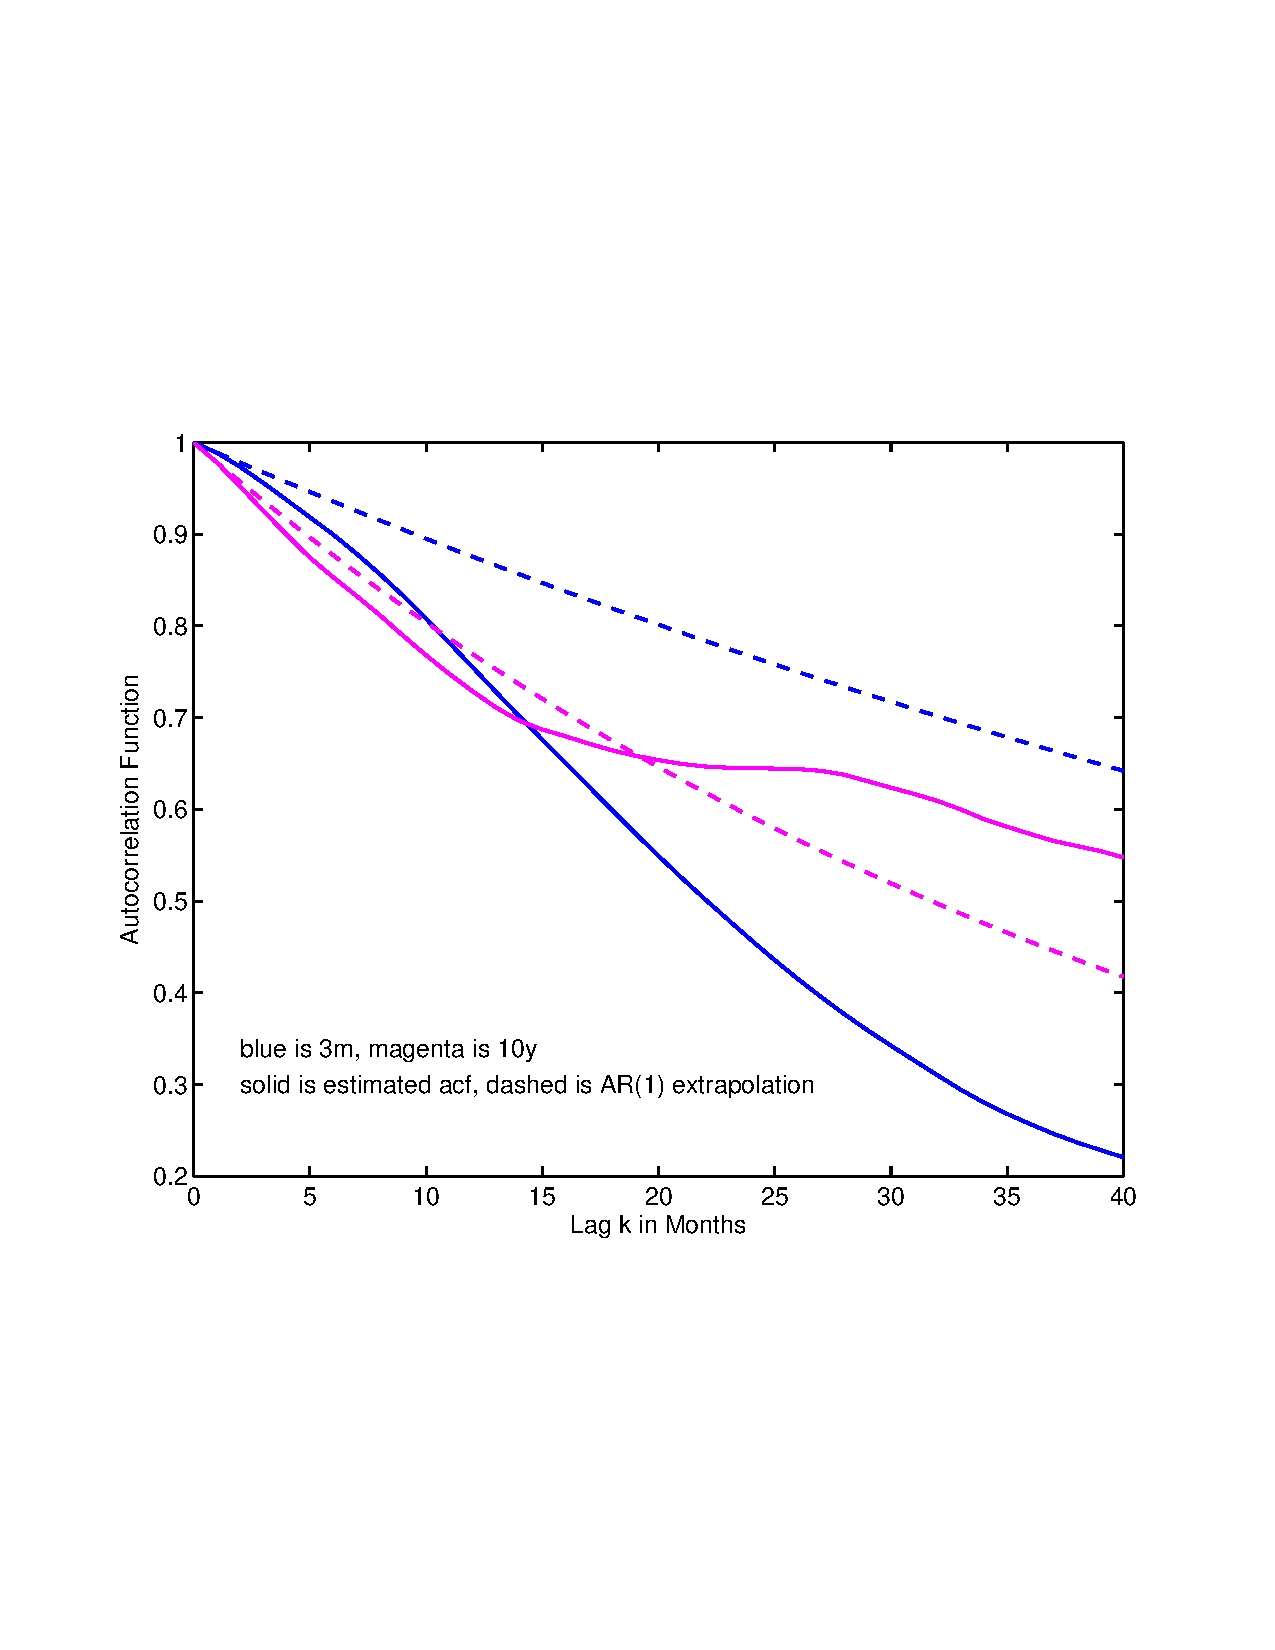
\includegraphics[width=4in]{../Matlab/hw7_q2.pdf}
%\end{center}

\item[(b)] With an AR(1), the autocorrelation has the form
$\rho(k) = \varphi^k$:  it declines geometrically.
If we set $\varphi = \rho(1)$, we can compute
estimated acf's corresponding to AR(1)s.
They're plotted as the dashed lines above.
You can see they're somewhat different from the AR(1).
Whether this represents sampling variability of some more
basic difference between the data and the AR(1) model isn't clear.


\end{enumerate}
\end{solution}

%-----------------------------------------------------------------------
\question {\it Dynamics of interest rates 2.\/}
Consider the barebones bond pricing model
based on the pricing kernel
\begin{eqnarray*}
    \log m_{t+1} &=& \delta + x_t + \lambda w_{t+1} \\
    x_{t}     &=& \sigma( w_{t} + \theta w_{t-1})  ,
\end{eqnarray*}
where $w_t$ is our usual iid normal disturbance
and $(\delta,\lambda,\sigma,\theta)$ are parameters.

\begin{parts}
\part What are the dynamics of $x_t$?
\part What is the moving average representation of $\log m_t$ in this model?
\part What is the variance of $x_t$?  Its first autocorrelation?
How does the autocorrelation function compare to the one
you computed for the 3-month treasury bill in the previous question?
\part Suppose the continuously-compounded short rate is $y^1_t = - \log q^1_t $.
What is $y^1_t$ in this model?
\end{parts}

\begin{solution}
\begin{parts}
\part It's an MA(1), which means it has a memory for one period only.
\part The log pricing kernel is an MA(2):
\begin{eqnarray*}
    \log m_t &=& \delta + \lambda w_t + \sigma (w_{t-1} + \theta w_{t-2}) .
\end{eqnarray*}\
\part The variance of $x_t$ (the variance of its stationary distribution)
is the sum of the squared MA coefficients:
\begin{eqnarray*}
    \mbox{Var}(x_t) &=& \sigma^2 + (\sigma\theta)^2 .
\end{eqnarray*}
The first autocovariance is
\begin{eqnarray*}
    \mbox{Cov}(x_t,x_{t-1}) &=& \sigma^2\theta ,
\end{eqnarray*}
so the first autocorrelation is the ratio,
$\rho(1) = \theta/(1+\theta^2)$.
All the autocovariances and autocorrelations after the first one are zero.
That's very different from what we see in the data,
where the autocorrelations declines more slowly.
\part Note that the distribution of $\log m_{t+1}$, 
conditional on the state at date $t$, is 
normal with mean $\delta + x_t$ and variance $\lambda^2$.
The one-period bond price is therefore 
\begin{eqnarray*}
    q^1_t &=& E_t (m_{t+1}) \;\;=\;\; \exp(\delta + x_t + \lambda^2/2) ,
\end{eqnarray*}
the usual ``mean plus variance over two'' formula.  
The one-period yield is 
\begin{eqnarray*}
    y^1_t &=& - \log q^1_t \;\;=\;\; - (\delta + x_t + \lambda^2/2) ,
\end{eqnarray*}
which is, by design, an MA(1).  



\end{parts}
\end{solution}


\end{questions}

\vfill \centerline{\it \copyright \ \number\year \
NYU Stern School of Business}

%\end{document}

\pagebreak
{\bf Matlab program:}
\verbatiminput{../Matlab/hw7_s13.m}

\end{document}


%  EXTRA STUFF


